\begin{figure}[H]
    \centering
    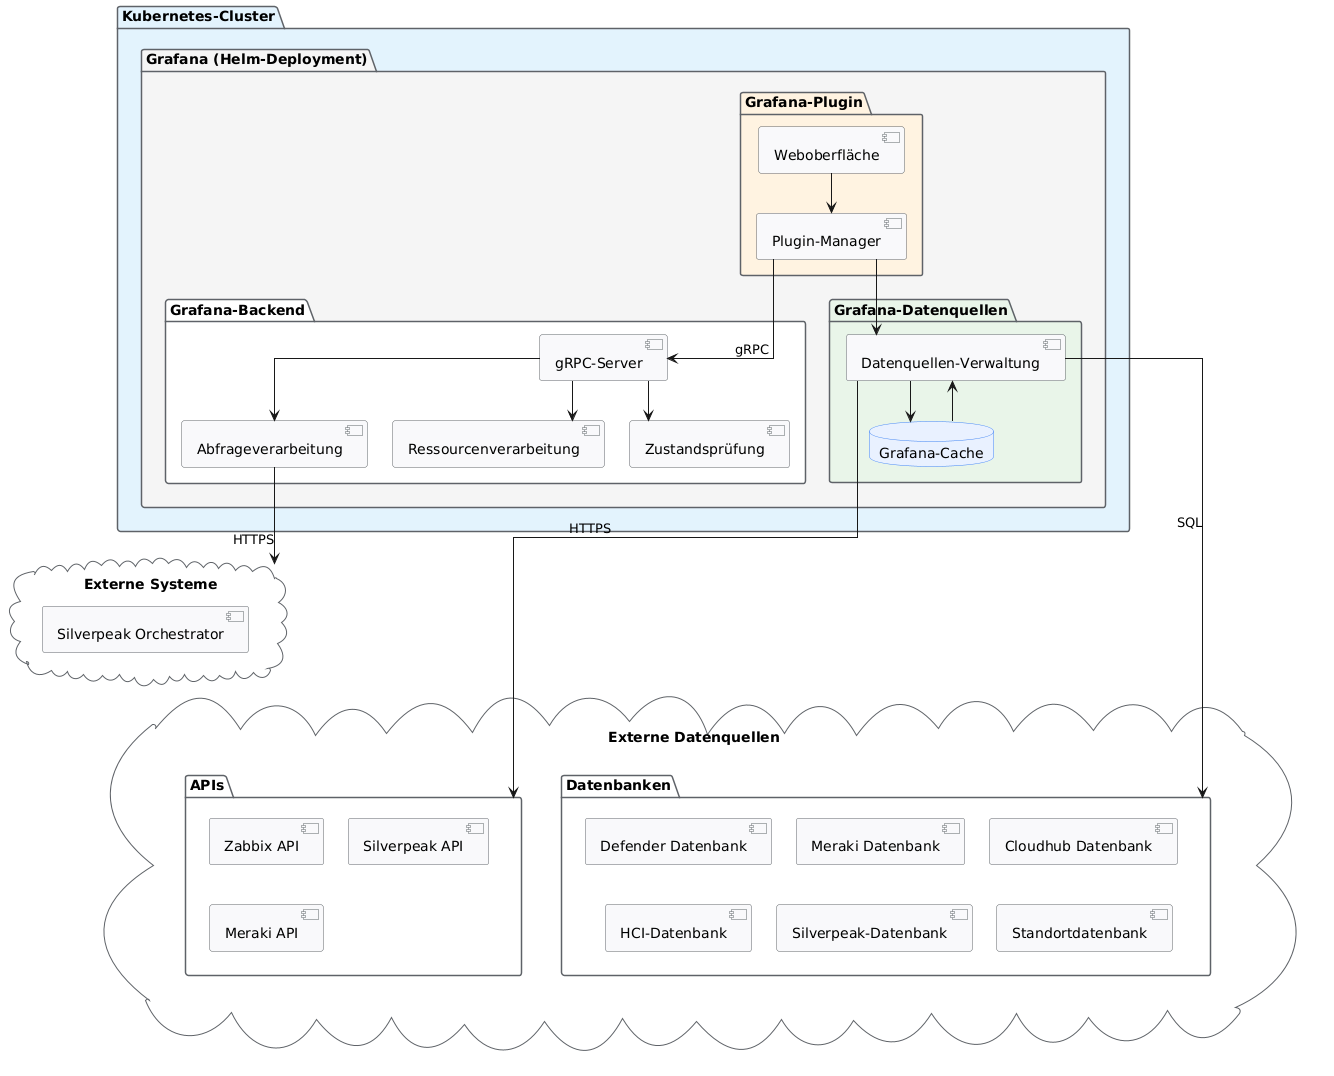
\includegraphics[width=\textwidth]{pics/datasource-architecture.png}
    \caption{Die Architektur des Grafana Plugins}
    \label{fig:datasource-architecture}
\end{figure}

Global Infrastructure Overview besteht aus einem selbstentwickelten \gls{grafana}-Plugin,
wie in Abschnitt~\ref{subsec:grafana-plugins} beschrieben. Ein eigenständiges Plugin wurde
gewählt, da die für diese Arbeit benötigte, standortbasierte und kartenartige Darstellung
mehrerer heterogener Datenquellen mit den standardmäßig verfügbaren \gls{grafana}-Panels
und -Datenquellen nicht abgebildet werden kann. Zur Entwicklung wurde das offizielle
\gls{grafana} Plugin SDK verwendet, das über die \gls{grafana} Plugin Tools bereitgestellt
wird~\cite{grafana2026plugintools}.

Dieses knüpft an die bestehende \gls{grafana}-Struktur an und nutzt bestehende Datenquellen,
die in Abschnitt~\ref{sec:defined-sources} beschrieben sind. Des Weiteren wurde das Plugin zu
einer bestehenden \gls{grafana}-Instanz hinzugefügt, die über \gls{helm} bereitgestellt wird,
wie in Abbildung~\ref{fig:datasource-architecture} dargestellt ist. Der Einsatz von \gls{helm}
ermöglicht dabei eine versionierte, wiederholbare Bereitstellung der \gls{grafana}-Instanz
über verschiedene Umgebungen hinweg~\cite{helm2026intro}.

Die einzelnen Systemelemente übernehmen folgende Aufgaben:
\begin{compactitem}
    \item \textbf{Weboberfläche:} Stellt die Konfigurations- und Anzeigeoberfläche des
    \gls{grafana}-Plugins innerhalb von \gls{grafana} bereit~\cite{grafana2026plugintools}.

    \item \textbf{Plugin-Manager:} Verwaltet den Lebenszyklus des Plugins und leitet
    Anfragen der Weboberfläche über \gls{grpc} an das Backend weiter~\cite{grafana2026backendplugins}.

    \item \textbf{gRPC-Server:} Nimmt die vom Plugin-Manager gesendeten Anfragen entgegen
    und verteilt sie an die zuständigen Backend-Komponenten~\cite{grafana2026backendplugins}.

    \item \textbf{Abfrageverarbeitung:} Verarbeitet Abfragen und ruft dafür Endpunkte der
    externen Systeme ab~\cite{grafana2026backendplugins}.

    \item \textbf{Ressourcenverarbeitung:} Stellt eigene, vom Plugin definierte
    HTTP-Ressourcen und -Endpunkte bereit~\cite{grafana2026backendplugins}.

    \item \textbf{Zustandsprüfung:} Überprüft die Verfügbarkeit und Funktionsfähigkeit
    des Plugins~\cite{grafana2026backendplugins}.

    \item \textbf{Datenquellen-Verwaltung:} Verwaltet den Zugriff auf die konfigurierten
    Datenquellen sowie den zugehörigen \gls{grafana}-Cache. Des Weiteren werden auch die statischen
    Zugangsdaten für die jeweiligen Datenquellen gehalten~\cite{grafana2026datasources}.

    \item \textbf{Grafana-Cache:} Speichert zwischenzeitlich abgerufene Daten, um wiederholte
    Anfragen an externe Systeme zu reduzieren. Bei einer erneuten, identischen Abfrage werden die
    Ergebnisse aus dem Cache anstelle der Datenquelle zurückgegeben~\cite{grafana2026datasourcecaching}.

    \item \textbf{Externe Systeme:} Umfassen unter anderem den Silverpeak Orchestrator, der
    über \gls{rest} angesprochen wird, wie in Abschnitt~\ref{subsec:silverpeak-api}
    beschrieben.

    \item \textbf{Externe Datenquellen:} Umfassen die APIs von Zabbix, Silverpeak und
    Meraki (siehe Abschnitte~\ref{sec:zabbix}, \ref{sec:silverpeak} und \ref{sec:meraki})
    sowie die zugehörigen Datenbanken, aus denen die überwachten Metriken und
    Konfigurationsdaten bezogen werden.
\end{compactitem}

Die Systemelemente, die über Grafana 

\section{Informationswege}
\label{sec:info-ways}

\section{Definierte Datenquellen}
\label{sec:defined-sources}

\section{Kubernetes}
\label{sec:kubernetes}